\usepackage[authoryear,round]{natbib}
\newcommand{\sheetnum}{%
	02
}
%\setcounter{section}{\sheetnum-3}
\newcommand{\tutorialtitle}{%
    Connectionist Neuron
}
\newcommand{\tutorialtitleshort}{%
	Perceptron
}
% for slides
\subtitle{\sheetnum \tutorialtitle}

\maxdeadcycles=1000 % Workaround for ! Output loop---100 consecutive dead cycles because of too many figures

% The following use of algroithms does not work well with the notes:
%
%
%
%
% instead use the following for your algorithms:
%
%\begin{figure}[!t]
%\removelatexerror
%\begin{algorithm}[H]
    % your aglo here
    %\label{alg:algolabel}
    %\caption{algocaption}
%\end{algorithm}
%\end{figure}
%\begin{algorithm}
% Below is the definition for the command \removelatexerror:
\makeatletter
\newcommand{\removelatexerror}{\let\@latex@error\@gobble}
\makeatother{}

\begin{document} %%%%%%%%%%%%%%%%%%%%%%%%%%%%%%%%%%%%%%%%%%%%%%%%%%%%%%%

\maxdeadcycles=1000 % Workaround for ! Output loop---100 consecutive dead cycles because of too many figures

\sheet{\sheetnum}{\tutorialtitleshort}

\ttopic{\tutorialtitle}

\columnratio{0.2,0.8}\textbf{}
\begin{paracol}{2}
%\setlength{\columnseprule}{0.1pt}
%\setlength{\columnsep}{5em}

\begin{rightcolumn}

% notes version will ignore it
\begin{frame}
\titlepage
\end{frame}

\begin{frame}
\tableofcontents
\end{frame}

\mode<all>
\section{Connectionist Neuron (Perceptron)}

\begin{frame}\frametitle{\secname}

A neuron is a computational unit for processing information. 

\question{What does a connectionist neuron compute?}\\

\pause
- A connectionist neuron is a type of neuron model which measures for a feature within an observation (a data point). It is a feature detector/extractor e.g. edge detector, above or below a threshold.

\end{frame}

\begin{frame}
A connectionist neuron's response to 1D data:

\begin{figure}[ht]
     \centering
     \savebox{\imagebox}{
	 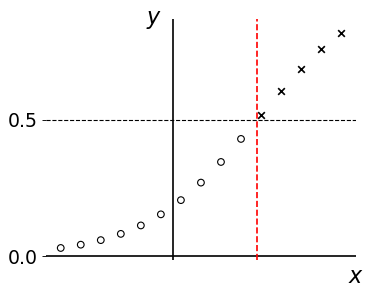
\includegraphics[width=0.3\textwidth]{img/neuron_1d_sigmoid.png}}%
     \begin{subfigure}[t]{0.35\textwidth}
         \centering
         \usebox{\imagebox}% Place largest image
         \caption{}
         \label{fig:neuron_1d_sigmoid}
     \end{subfigure}
     \hspace{10mm}
     \begin{subfigure}[t]{0.35\textwidth}
         \centering
         \raisebox{\dimexpr.5\ht\imagebox-.5\height}{% Raise smaller image into place
         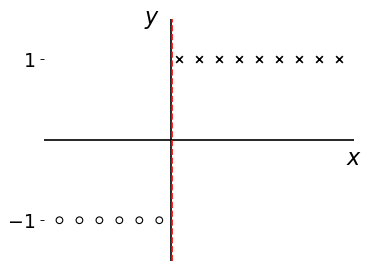
\includegraphics[width=0.9\textwidth]{img/neuron_1d_sign.png}
         }
         \caption{}
         \label{fig:neuron_1d_sign}
     \end{subfigure}
     \mode<article>{
     \caption{Examples of different neuron responses to scalar input of two types: $\times$ and $\circ$. In \ref{fig:neuron_1d_sigmoid}: The neuron's response $y$ is continuous. In \ref{fig:neuron_1d_sign} the neuron repsonse is $+1$ for positive input and $-1$ otherwise. The red lines act as a decision boundary.}
	 }
	 \label{fig:neuron_1d}
\end{figure}

\end{frame}

\begin{frame}\frametitle{
A connectionist neuron's response to 3D data:}

\begin{figure}[ht]
     \centering
	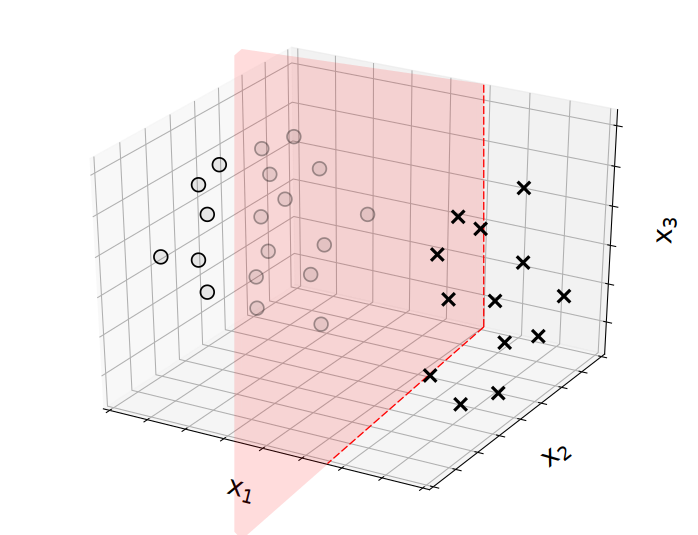
\includegraphics[width=0.4\textwidth]{img/neuron_3d_grid}
     \mode<article>{
	\caption{Examples of a neuron's response to 3D input of types $\times$ and $\circ$. Inputs of different types fall on opposite sides of a plane. The red plane acts as a decision boundary}
	}
	\label{fig:neuron_3d_grid} 
\end{figure}
\end{frame}

\subsection{Components of the connectionist neuron}
    
\begin{frame}
    
    \begin{figure}[h]
        \centering
        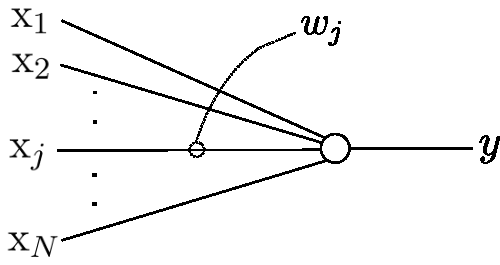
\includegraphics[height=2.5cm]{img/linearNeuron_y.pdf}
        \caption{The input-output relationship for a connectionist neuron. $w_{j}$ describes the connection from the $j$-th input.}
        \label{fig:neuron_diagram}
    \end{figure}
    \notesonly{
    \figref{fig:neuron_diagram} is a diagram of a connectionist neuron.} Given an input vector $\vec x \in \R^{N}$ with components $x_{j}$,
    the connectionist neuron is composed of the following elements:

    \begin{enumerate}[(a)]
        \item weights $\vec w \in \R^{N}$\notesonly{: The weights represent the strength of the connections between the neuron and each component of the input it receives.}\\
        \item A linear filter: \notesonly{Summation of the weighted inputs, i.e. scalar product: }$\vec w^{\top} \vec x = \sum_{j} w_{j} x_{j}$.
        \item A bias value $\theta \in \R$ also known as the \emph{threshold} of the neuron.
        \item An activation function or transfer function $f: \R \mapsto \R$. \\
        \mode<article>{
        
        $f(\cdot)$ controls the range of the neuron's response. It can have the effect of squashing the response to a specific range of values or a specific set of values and preventing other value ranges.
        }
        \item The scalar output of the neuron: $y$.
    \end{enumerate}
    
    \question{How does one interpret the scalar product $\vec w^\top \vec x$?}\\
    
    \mode<article>{
    The scalar product (dot product) acts as measure of similarity between $\vec w$ and $\vec x$.
    By looking at the geometric interpretation of the scalar product (dot product):
    \begin{equation}
    \vec w\top\vec x = ||\vec w||\;||\vec x||\,\cos{\beta}
    \end{equation}
    
    where $\beta$ is the angle between the two vectors. Therefore, $\vec w^\top \vec x$:
    
    \begin{itemize}
    \item is maximal when both vectors point in the same direction.
    \item It is zero if both vectors are orthogonal.
    \item It is maximally negative when both vectors point in opposite direction.
    \end{itemize}
    }
   
\end{frame}
\begin{frame}
    
    \begin{figure}[h]
        \centering
        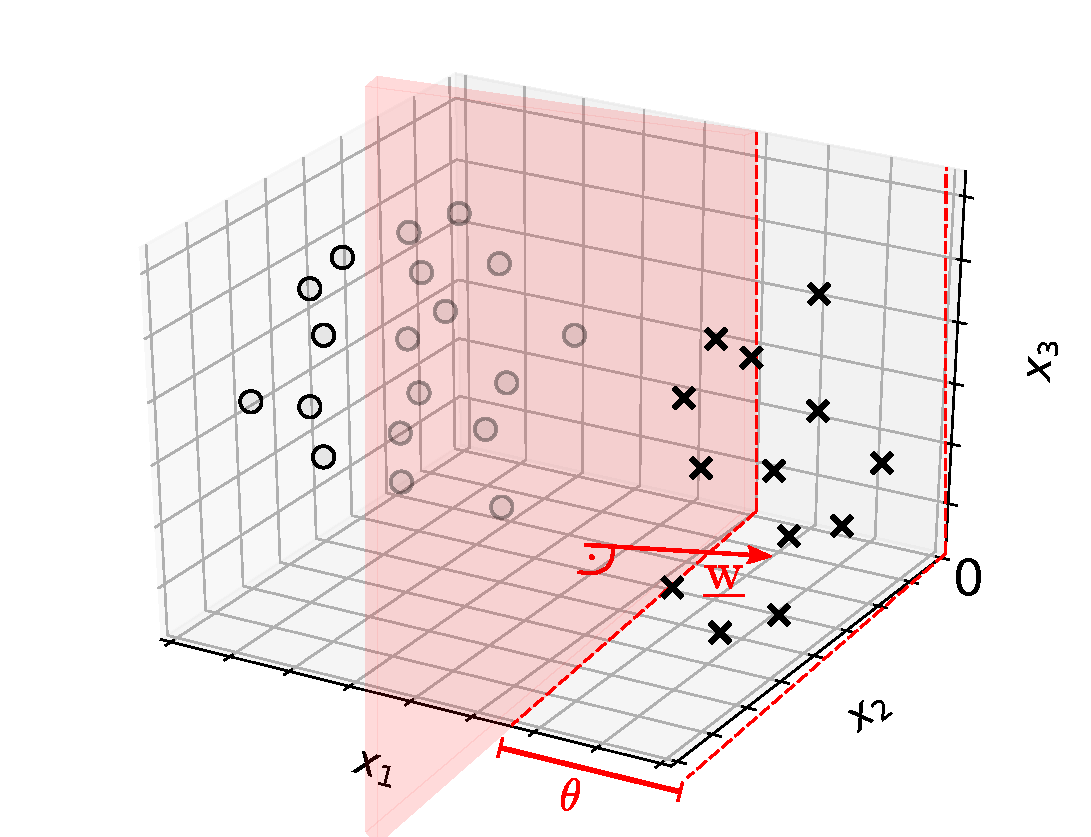
\includegraphics[height=6cm]{img/neuron_3d_grid_hyperplane.pdf}
        \caption{The plane divides the responses of the neuron. In the context of classification it is referred to as the decision boundary.}
        \label{fig:neuron_3d_grid_hyperplane}
    \end{figure}
    
\end{frame}
\begin{frame}
    
    The input-output relationship is described by a linear filter with a static non-linearity $f(\cdot)$:

    \begin{equation}
        \label{eq:linearNeuron}
        y = f \Big(\; \underbrace{\sum_{j=1}^{N} {w}_{j} 
            {x}_j - \theta}_{=:h} \; \Big)
            = f \big(\;  \vec{w}^{\top}
            \vec{x}- \theta \; \big)
            = f(\,h\,)
    \end{equation}
    
	\[ \begin{array}{ll} 
		\vec{x}: & \text{input vector with components } \mathrm{x}_j \\
		y: & \text{scalar output of the neuron } \\
		\vec{w}: & \text{weight vector of the neuron with components }
			\mathrm{w}_{j}\\
		\theta: & \text{threshold of the neuron} \\
		h: & \text{total input of the neuron. } \\
		&\quad h \propto \frac{\vec w^\top \vec x}{\;||\vec w||_2} \text{ component of $\vec x$ in the direction of $\vec w$}\\
		f(\cdot): & \text{transfer function}
	\end{array} \]
    
\end{frame}

\begin{frame}

\question{What roles do the weights and bias play?}

\pause
{}
\mode<article>{
\begin{itemize}
\item[-] $\vec w$ is effectively the normal vector of the hyperplane $\color{red}H = \{\vec x : \vec w^{\top} \vec x = \theta\}$. Therefore, the weights represent the orientation of the hyperplane (see. \figref{fig:neuron_3d_grid_hyperplane}).
\item[-] $\theta$ represents the shift of the hyperplane (see. \figref{fig:neuron_3d_grid_hyperplane}). It is the absolute position of the hyperplane fron the origin along $\vec w$. For any point $\widetilde{\vec x} \in H$ (i.e. points on the plane): 
$\frac{\vec w^\top \widetilde{\vec x}}{\,||\vec w||_2} = \frac{\theta}{\,||\vec w||_2}$
\end{itemize}
}

\mode<presentation>{
    \begin{figure}
        \centering
        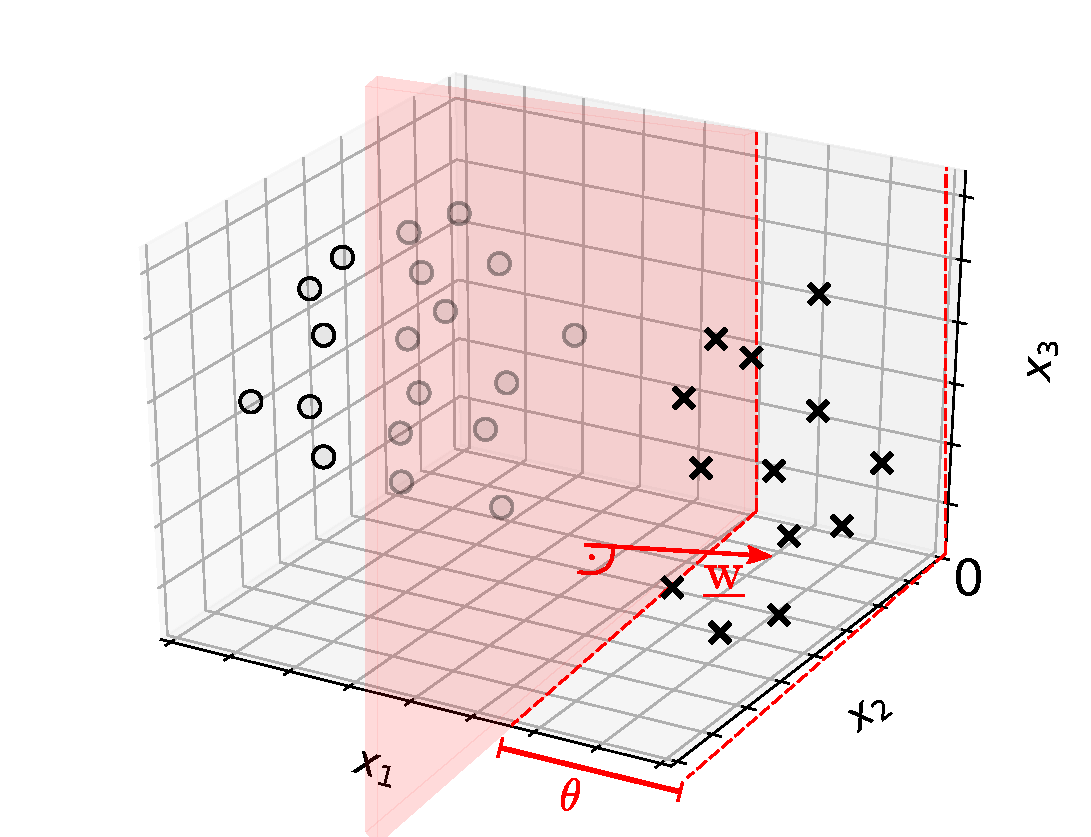
\includegraphics[height=6cm]{img/neuron_3d_grid_hyperplane.pdf}
    \end{figure}
}
\end{frame}

\subsection{Linear vs. non-linear transfer functions}

\begin{frame}


\question{What are the advantages of using a non-linear transfer function instead of a linear one?}

\begin{figure}[ht]
     \centering
     \savebox{\imagebox}{
	 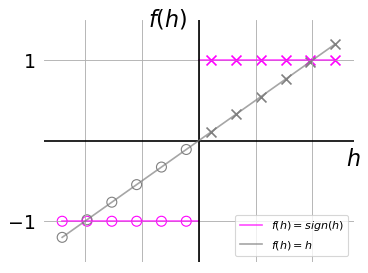
\includegraphics[width=0.3\textwidth]{img/neuron_1d_sign_and_linear}}%
     \begin{subfigure}[t]{0.35\textwidth}
         \centering
         \usebox{\imagebox}% Place largest image
         \caption{\footnotesize Linear vs. non-linear activation}
         \label{fig:linear_sign}
     \end{subfigure}
     \hspace{2mm}
     \begin{subfigure}[t]{0.35\textwidth}
         \centering
         \raisebox{\dimexpr.5\ht\imagebox-.5\height}{% Raise smaller image into place
         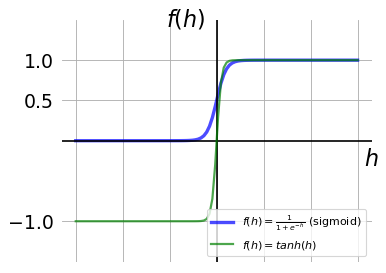
\includegraphics[width=0.9\textwidth]{img/neuron_1d_sigm_tanh}
         }
         \caption{\footnotesize logistic sigmoidal $\scriptstyle f(h)=\frac{1}{1+e^{-h}}$ vs. tanh}
         \label{fig:sigmoid_tanh}
     \end{subfigure}
     \mode<article>{
     \caption{Comparing linear with non-linear activation functions and differentiable alternatives to the sign function.}
     }
	 \label{fig:transfer_linear_nonlinear}
\end{figure}

\pause
- Advantages:
\begin{enumerate}
\item binary classification, either $f(h) \in \{0,1\}$ or $f(h) \in \{-1,1\}$
\item interpret $f(h)$ as a probability. The logistic sigmoidal where $f(h) = \frac{1}{1+exp(-h)}$ yields values in the range of (0,1). The logistic sigmoidal can also be obtained by shifting and scaling the tanh function (see \sectionref{sec:tanh_to_sigmoid}.
\item a multilayer perceptron with only linear transfer functions can be reduced to a single layer. The hidden layers become redundant \footnote{Recent literature reveals interesting insights in what kind of representations are found across the layers of linear networks. For more information see Saxe, A. M., McClelland, J. L., \& Ganguli, S. (2019). A mathematical theory of semantic development in deep neural networks. Proceedings of the National Academy of Sciences, 116(23), 11537-11546.}:\\

     \begin{tabular}{c c c }
     		\raisebox{-9mm}{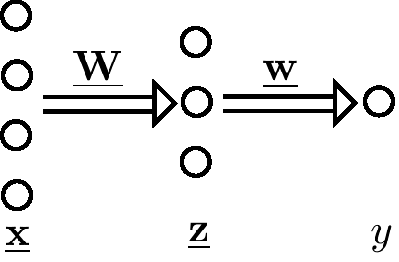
\includegraphics[height=2.25cm]{img/section1_fig16.pdf}}
     	& 
     		\begin{minipage}{10mm}
     			\vspace{10mm}
     		\end{minipage} 
     	& 
     		\parbox{4cm}{
		    \begin{eqnarray*}
		      y & = & \vec{w}^\top \vec{z}  
		      \quad = \quad \vec{w}^\top \vec{W} \, \vec{x} \\
		      & = & (\underbrace{\vec{W}^\top \vec{w}}_{=: \widehat{\vec{w}}})^\top \vec{x}
		      \quad = \quad \widehat{\vec{w}}^\top \vec{x}\\ 
		      & \corresponds & \text{connectionist neuron}
		    \end{eqnarray*}}
	\end{tabular}
\end{enumerate}


\end{frame}

\begin{frame}

\question{How does the logistic sigmoidal function relate to the tanh function?}

\mode<presentation>{

	\only<1,2>{\placeimage{9.5}{4}{img/neuron_1d_sigm_tanh}{width=4.cm}}
}

\mode<article>{

We observe in \figref{fig:sigmoid_tanh} that the logistic sigmoidal function (sigmoid) function is a shifted and scaled variant of the tanh function.
}

From this follows:
	\begin{align}
	f_{{\text{sigmoid}}}(h) 
    & = \frac{1}{1 + e^{-h}} \\
	& = \frac{e^{\frac{h}{2}}}{e^{\frac{h}{2}} + e^{-\frac{h}{2}}} \\
	& = \frac{1}{2} \Bigg(
		\underbrace{\frac{e^{\frac{h}{2}} - e^{-\frac{h}{2}}}{
			e^{\frac{h}{2}} + e^{-\frac{h}{2}}}}_{
				= \tanh \frac{h}{2}}
		+ \underbrace{\frac{e^{\frac{h}{2}} + e^{-\frac{h}{2}}}{
				e^{\frac{h}{2}} + e^{-\frac{h}{2}}}}_{= 1}
		\Bigg) \\
	& = \frac{1}{2} \left( \tanh \frac{h}{2} + 1 \right)
	\end{align}

    
\end{frame}

\subsection{Shortcut notation for weights and bias}

\begin{frame}

\mode<article>{
The bias is effectively a connection between the neuron and an input that is always on. 
We can absorb the bias into the weight vector by prepending it to $\vec w$ and prepending $\vec x$ with an element $x_0 = 1$:
}

    \begin{figure}[h]
        \centering
        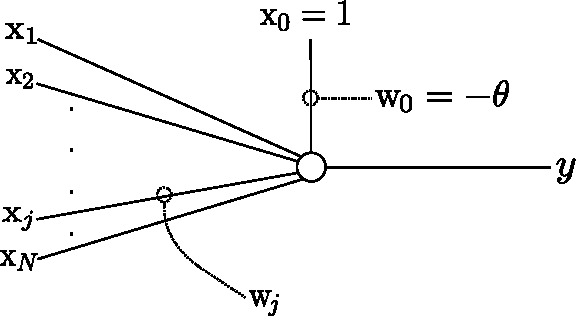
\includegraphics[height=3cm]{img/section1_fig6}
         \caption{Absorb bias into weight vector.}
         \label{fig:weight_with_bias}
    \end{figure}
 
\only<1>{
\mode<article>{   
The response of the neuron depicted in \figref{fig:weight_with_bias} can be computed by:
}

\begin{equation}
	y = f\big( \sum_{{\color{blue}j=0}}^{N} \mathrm{w}_j \mathrm{x}_j \big)
		= f( \vec{w}^\top \vec{x} )
	\label{eq:weight_with_bias}
\end{equation}

\mode<article>{

Note that the sum in \eqref{eq:weight_with_bias} now iterates from ${\color{blue}j=0}$ instead of $j=1$ as was done in \eqref{eq:linearNeuron} in order to include the bias element.
}

}

\only<2>{


	$\vec{w}$ will be used for $\rmat{ \mathrm{w}_1 \\ \vdots\;\,\\ \mathrm{w}_N}$ 
	as well as for $\rmat{ \mathrm{w}_0 \\ \mathrm{w}_1 \\ \vdots\;\, \\ \mathrm{w}_N}$. \\
	
	\rule{2cm}{0pt}
	
	Accordingly,
	$\vec{x}$ will be used for $\rmat{ \mathrm{x}_1 \\ \vdots\;\,\\ \mathrm{x}_N}$ 
	as well as for $\rmat{ \mathrm{x}_0 \\ \mathrm{x}_1 \\ \vdots\;\,\\ \mathrm{x}_N}$.
	
	\mode<article>{
	Whether the bias is absorbed or not should become apparent from the context or explicitly from the limits of the sum.
	}
}

\end{frame}

\mode*

\clearpage

\mode<all>
\section{Limitations of Perceptrons}

\mode<presentation>{
\begin{frame} 
    \begin{center} \huge
        \secname
    \end{center}
    \begin{center}
    From neurons to neural networks
    \end{center}
\end{frame}
}

\mode<article>{
Connectionist neurons, or perceptrons, are limited in the variety of functions they are able to fit. 
When dealing with classification problems, a perceptron can only find a linear separation between any two classes. Irrespective of the neuron's non-linear activation function, the perceptron is regarded as a \emph{linear classifier}. Whether something falls on one side of the decision boundary or the other, is entirely based on applying a linear filter (i.e. $\vec w^{\top} \vec x$). The non-linearity $f(h)$ merely controls the value range of the neuron's response ($\{0,1\}, (-1,+1)$, \ldots) which helps in interpreting the neuron's response.\\

If observations for two different classes are distributed such that one cannot draw a line to separate them, then the two classes
are not linearly separable. In this case, the perceptron will fail to find a suitable classification boundary between the two classes.
}

\begin{frame}\frametitle{Linear classifiers/linear decision boundaries}

Consider the following binary classification problems with $\vec x \in \R^2$.{}

\question{Can you find a line that separates the two classes for each case?}

\begin{figure}[h]
    \centering
	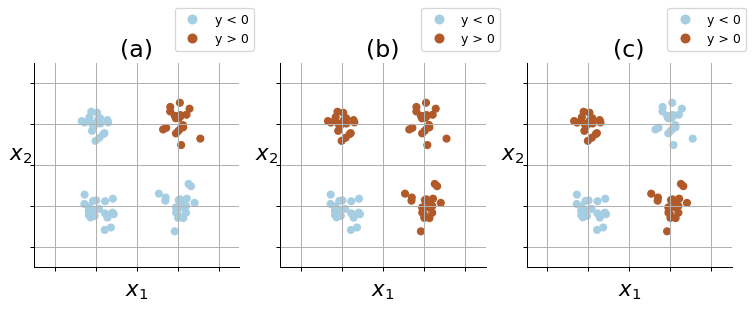
\includegraphics[width=0.8\textwidth]{img/and_or_xor_y}
	\mode<article>{
	\caption{(a) points are classified according to the AND function,
	(b) points are classified according to the OR function,
	(c) points are classified according to the XOR function.
	}
	}
	\label{fig:and_or_xor} 
\end{figure}

\mode<article>{
In \figureref{fig:and_or_xor}, particularly (a) and (b),
it is possible to draw a line that separates the classes. Therefore, the AND and OR functions are linearly separable.
A perceptron is capable of finding such a separating line. However, this does not apply to the third case, for the XOR function.
It is impossible to find a single line that will separate the classes.\\
The XOR function is not linearly separable.
}

\pause 

\question{Can we solve the XOR problem with multiple perceptrons? How?}\\

%\slidesonly{
%\begin{figure}[ht]
     %\centering
	%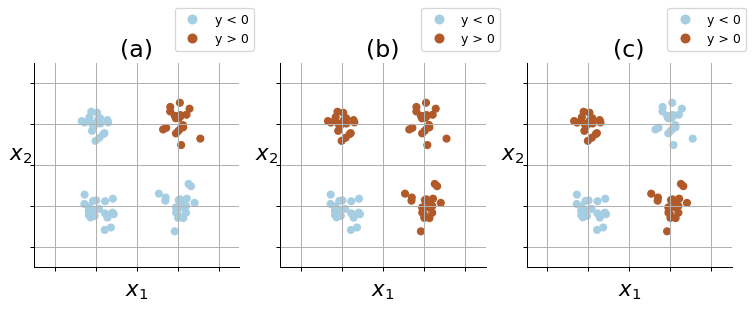
\includegraphics[trim=480 0 0 30, clip, width=0.4\textwidth]{img/and_or_xor_y.png}
	%\caption*{A single perceptron can not solve the XOR problem.}
	%\label{fig:xor} 
%\end{figure}
%}

\pause

\notesonly{
- Yes, think of it as a divide and conquer approach. We split the XOR problem into multiple sub-problems. 
A perceptron is used to solve each sub-problem.

If you're familiar with Boolean algebra, you might recognize the following expression for the XOR function:
}
\mode<presentation>{
\vspace{-10mm}
}

\begin{equation}
\label{eq:xor}
\mathrm{XOR}(x_1, x_2) = 
({\color{magenta}\,{x_1} \; \mathrm{AND} \; \overline{x}_2 \,})
 \;\; \mathrm{OR} \;\; 
({\color{green}\, \overline{x}_1 \; \mathrm{AND} \; x_2 \,})
\end{equation}

\end{frame}

\begin{frame}{Inversion/NOT-Gate}

\begin{center}
\begin{minipage}{0.9\textwidth}

\begin{center}
\begin{minipage}{0.45\textwidth}
	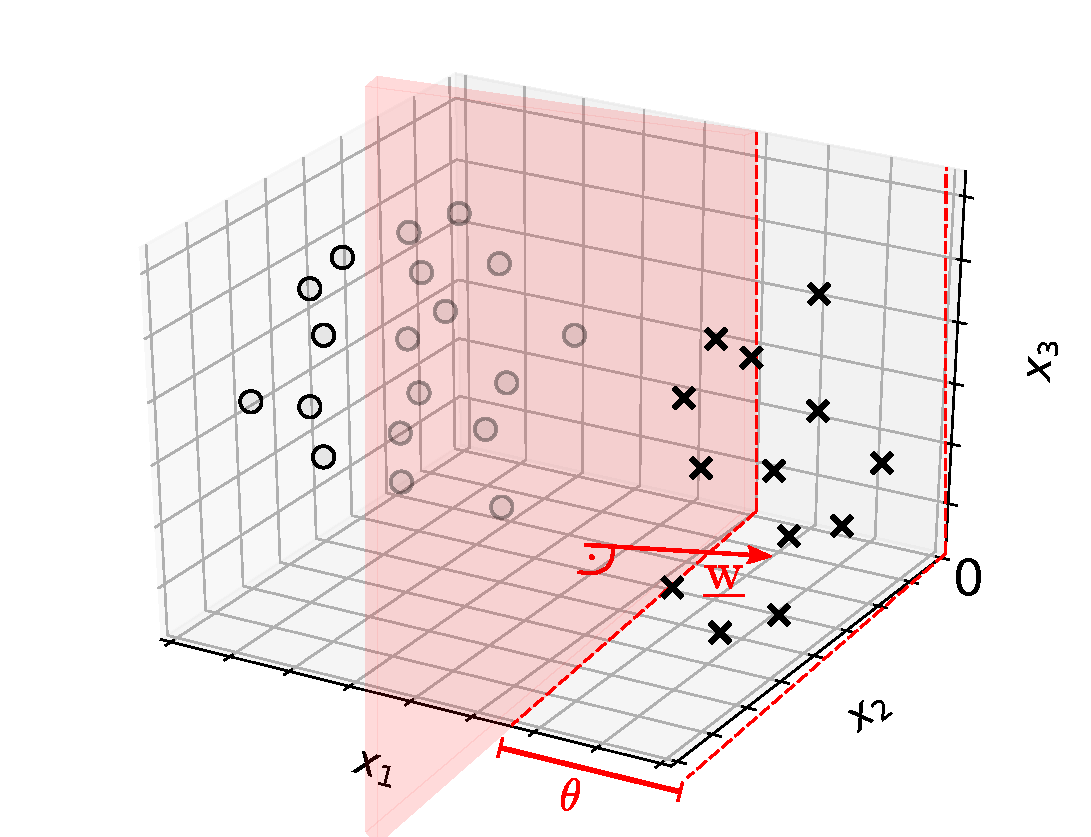
\includegraphics[width=0.9\textwidth]{img/neuron_3d_grid_hyperplane}
\end{minipage}
\begin{minipage}{0.45\textwidth}
	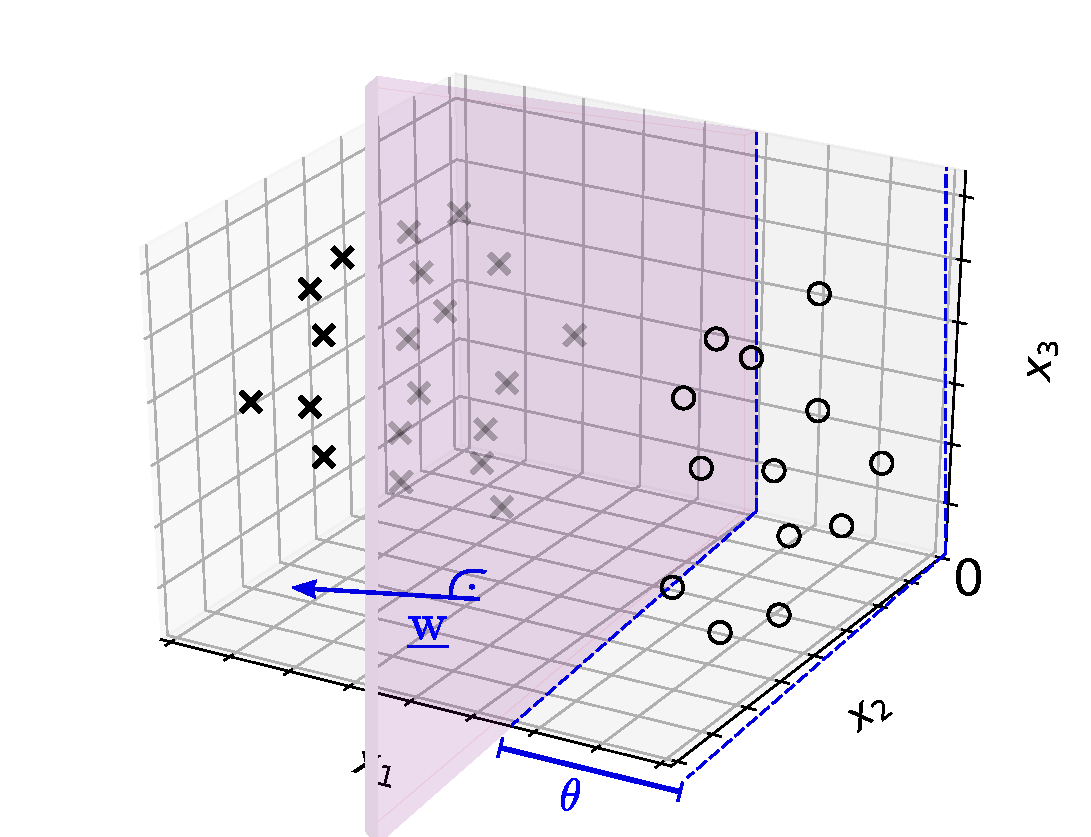
\includegraphics[width=0.9\textwidth]{img/neuron_3d_grid_hyperplane_flip}
\end{minipage}

\end{center}
\end{minipage}
\captionof{figure}{Inverting a neuron's response by flipping the hyperplane}
\end{center}

\end{frame}


\mode<article>{
For instance, the first perceptron ${\color{magenta}s^1_1}$ is tasked to separate the bottom-right cloud of points from the rest. 
A second perceptron ${\color{green}s^1_2}$ is used to separate the top-left cloud from the rest.
A third perceptron ${\color{blue}s^2_1}$ will then use the responses of both and respond to ``is \textbf{only one} of the two perceptrons \textbf{on}?''.

\figref{fig:build_xor} illustrates this approach. One need only recognize that each sub-problem is linearly separable.\\
}

\begin{frame}

\slidesonly{
\begin{equation}
\label{eq:xor}
\mathrm{XOR}(x_1, x_2) = 
({\color{magenta}\,{x_1} \; \mathrm{AND} \; \overline{x}_2 \,})
 \;\; \mathrm{OR} \;\; 
({\color{green}\, \overline{x}_1 \; \mathrm{AND} \; x_2 \,})
\end{equation}
}

\begin{figure}[ht]
    \centering
	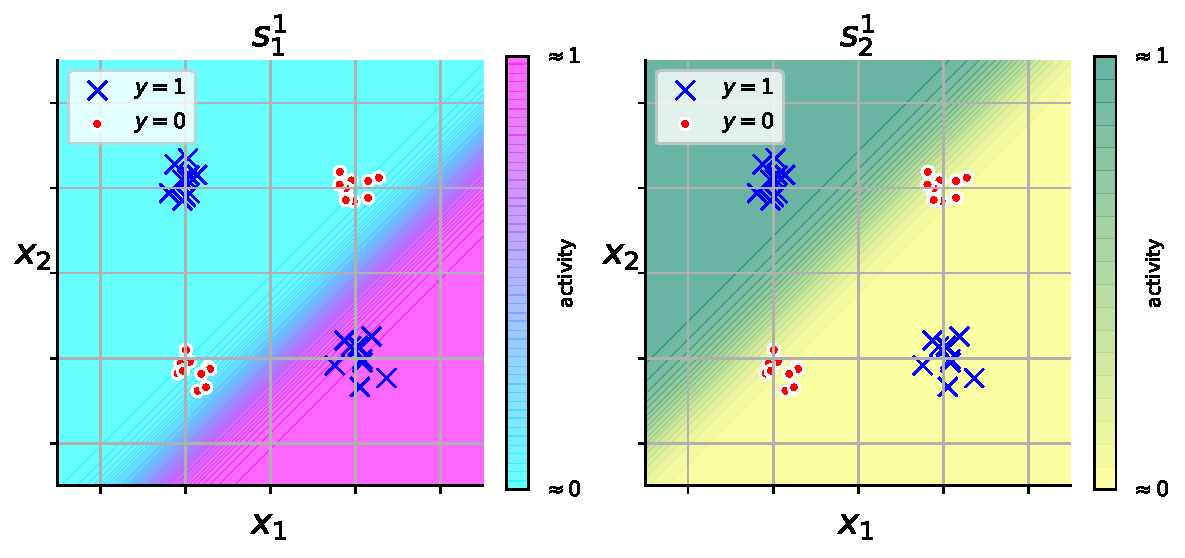
\includegraphics[width=0.75\textwidth]{img/build_xor_crf}
	\caption{Solving sub-problems of the XOR problem.}
	\label{fig:build_xor} 
\end{figure}

\end{frame}

\begin{frame}

\begin{figure}[ht]
    \centering
	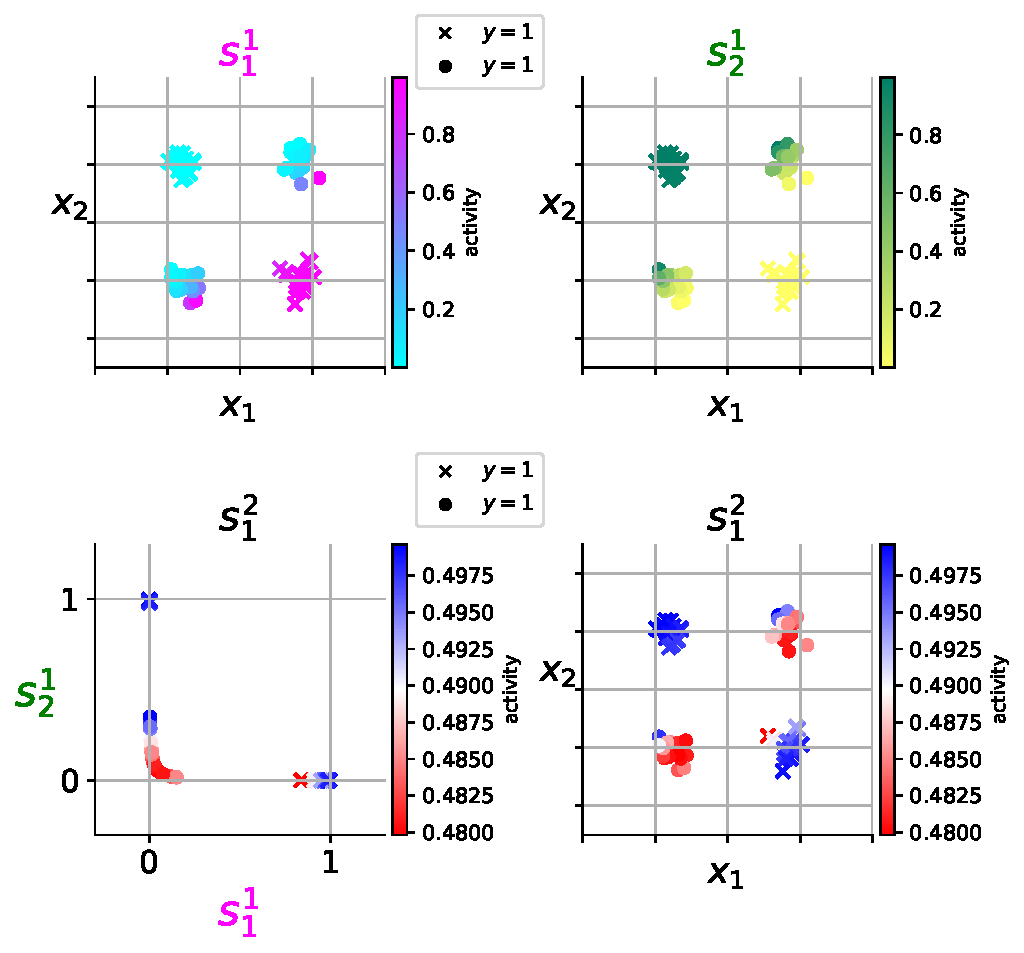
\includegraphics[width=0.75\textwidth]{img/build_xor}
	\caption{Solving sub-problems of the XOR problem.}
	\label{fig:build_xor} 
\end{figure}

\end{frame}


\mode<article>{
\figref{fig:xor_decisions} visualizes the response of the final neuron $s^2_1$ for different values of $x_1$ and $x_2$. The space is partitioned into one region in which the activity is $< 0.5$ and two disjoint regions (top-left \& bottom-right) in which the activity is $> 0.5$.
}

\begin{frame}
\begin{figure}[ht]
     \centering
     \savebox{\imagebox}{
     \mode<presentation>{
	 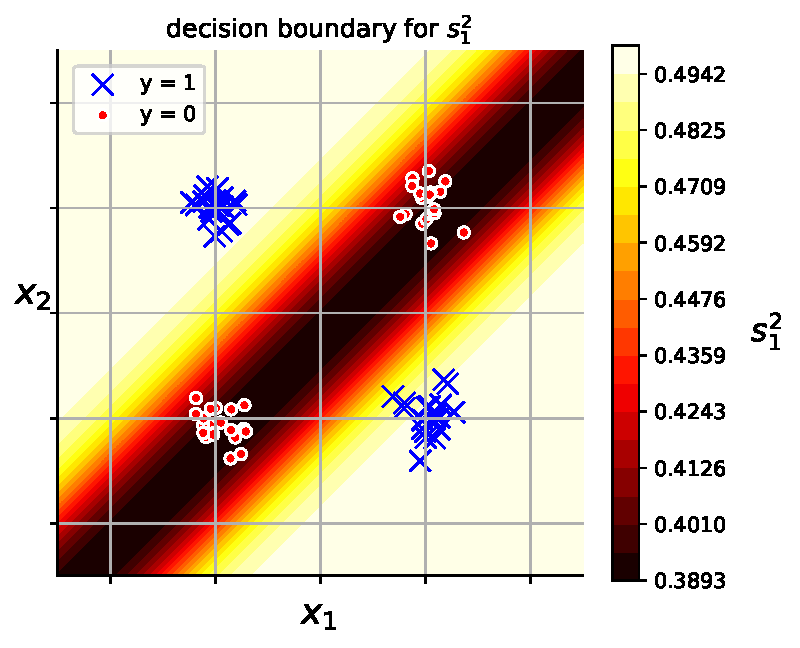
\includegraphics[width=0.4\textwidth]{img/xor_decision}
	 }
     \mode<article>{
	 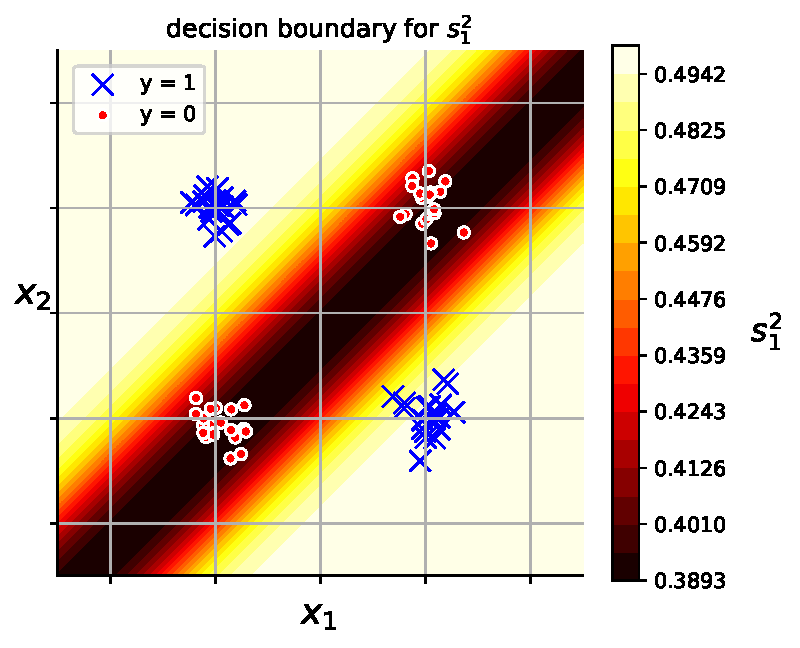
\includegraphics[width=0.35\textwidth]{img/xor_decision}
	 }
	 }%
     \begin{subfigure}[t]{0.35\textwidth}
         \centering
         \usebox{\imagebox}% Place largest image
         \caption{}
         \label{fig:xor_decisions}
     \end{subfigure}
     \slidesonly{
     \hspace{4mm}
     \begin{subfigure}[t]{0.45\textwidth}
     }
    \notesonly{
     \hspace{1mm}
     \begin{subfigure}[t]{0.38\textwidth}
     }
         \centering
         \raisebox{\dimexpr.5\ht\imagebox-.5\height}{% Raise smaller image into place
         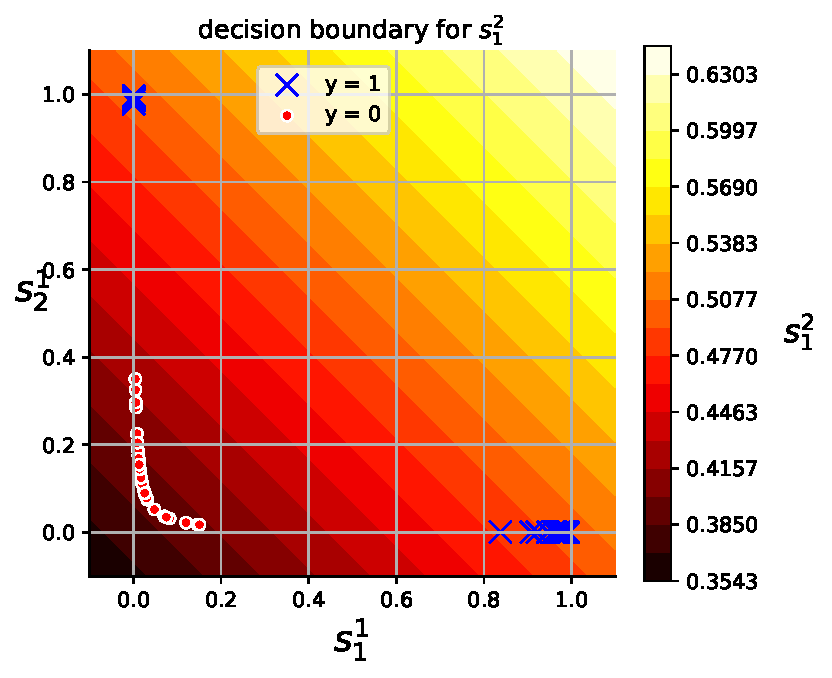
\includegraphics[width=0.9\textwidth]{img/xor_decision_s}
         }
         \caption{}
         \label{fig:xor_decisions_s}
     \end{subfigure}
	\caption{Identifying the decision boundaries.}
\end{figure}
\end{frame}

\newpage
\mode<article>{


What we are essentially describing is a Multilayered perceptron (MLP) with an architecture as illustrated in \figref{fig:xor_mlp_arch}. This MLP is made up of an output layer with a single output neuron ${\color{blue}s^2_1}$, and one hidden layer with two hidden neurons, ${\color{magenta}s^1_1}$ and ${\color{green}s^1_2}$ (the superscript denotes the layer index, the subscript denotes the neuron index within its layer). The terms ``neurons'' and ``nodes'' are treated as synonyms.
}
\begin{frame}

\begin{figure}[ht]
    \centering
	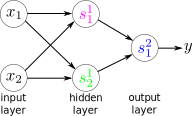
\includegraphics[width=0.4\textwidth]{img/xor_mlp_arch}
	\caption{simplified MLP architecture}
	\label{fig:xor_mlp_arch} 
\end{figure}



\end{frame}



\mode*

\section{References}
\begin{frame}[allowframebreaks] \frametitle{References}
	\scriptsize
	\bibliographystyle{plainnat}
	\bibliography{bibliography}
\end{frame}

\end{rightcolumn}
\end{paracol}

\end{document}
